\documentclass[conference]{IEEEtran}
\IEEEoverridecommandlockouts
\renewcommand{\refname}{Bibliografía}
% The preceding line is only needed to identify funding in the first footnote. If that is unneeded, please comment it out.
\usepackage{cite}
\usepackage{amsmath,amssymb,amsfonts}
\usepackage{algorithmic}
\usepackage{graphicx}
\usepackage{textcomp}
\usepackage{xcolor}
\usepackage{url}
\usepackage{upgreek}
\usepackage{amssymb}
\usepackage{verbatim}
\def\BibTeX{{\rm B\kern-.05em{\sc i\kern-.025em b}\kern-.08em
    T\kern-.1667em\lower.7ex\hbox{E}\kern-.125emX}}
\begin{document}

\title{Proyecto 3\\
{\footnotesize \textsuperscript{}IC3002 - Análisis de Algoritmos}
{\footnotesize \textsuperscript{}Profe.: Yuen Law Wan}
{\footnotesize \textsuperscript{}I Semestre 2020}
}

\author{\IEEEauthorblockN{Joseph Tenorio Pereira}
\IEEEauthorblockA{\textit{2019064588} \\
}
\and
\IEEEauthorblockN{Jose Pablo Muñoz Montero}
\IEEEauthorblockA{\textit{2019061904} \\
}
}

\maketitle

\begin{abstract}
The following documentation revolves around the desing, analysis, and \textit{Python} implementation of a Genetic Algorithm whose purpose is to produce simulated robots capable of solving a given maze. The aforementioned robots are to have certain simulated properties suchs as hardware, cost and behaviour, and it is through these characteristics that the Genetic Algorithm is expected to generate better robots with each iteration. All parts of the creation of a Genetic Algorithm will be discussed as part of the design, that includes chromosome and adaptability function definition, selection, mutation and crossover. Aditionally, the behaviour property is to be dictated by a Markov Chain representation, so the combination of Genetic Algorithms and Markov Chains is briefly covered. Finally, results of the implementation will be shown, emphasizing the difference between the firsts and lasts generations, and conclusions will be drawn.
\end{abstract}

\section{Introducción}

Los algoritmos genéticos se entienden, según \cite{b1}, como un tipo de algoritmo evolutivo en el que representaciones de posibles soluciones, llamadas genes o cromosomas, son puestos a prueba, cruzados y mutados con el fin de llegar a genes mejor adaptados, es decir, soluciones óptimas. El cruce y selección de genes es hecho con base en la selección natural biológica, de hecho, los algoritmos genéticos en general están inspirados en dicho mecanismo evolutivo. Otro ejemplo de lo anterior es la introducción de mutaciones a los genes, es decir, cambiar aleatoriamente los valores de los mismos, de modo que  se cuente con un minímo de aleatoriedad en el algoritmo. Los componentes más importantes del diseño de un algoritmo genético suelen ser la definición, selección y cruce de los cromosomas, y son precisamente estos componentes del algoritmo los que seran discutidos en el presente documento. Cabe señalar que la función de adaptabilidad del algoritmo, aquella formula por medio de la cual se determinan cuáles soluciones son más deseables que otras, es también discutida durante el proyecto. 

Otro concepto a tener en cuenta en el presente proyecto es el de cadenas de Markov, las cuáles de acuerdo a \cite{b2} se suelen explicar como un conjunto de propiedades juntadas y representadas como un estado (aquí llamados "nodos") y las probabilidades de que el proceso representado por la cadena pase de un estado a cualquier otro (aquí llamados "arcos"). Cabe resaltar que las cadenas de Markov son una forma de representar los procesos de Markov y estos últimos tienen la propiedad fundamental de que la probabilidad de pasar de un estado a otro depende únicamente del estado actual. Tomando en cuenta lo anterior, es posible describir y estimar una predicción de una amplia gama de comportamientos por medio de cadenas de Markov, ya que es posible representar dicho comportamiento como una serie de recorridos a lo largo del tiempo entre los estados, donde la elección del siguiente estado es dictada por la probabilidad entre dicho estado y el actual.

El presente proyecto busca diseñar un algoritmo genético capaz de producir robots eficientes en la resolución de un laberinto dado. Para ello se requiere, además del algoritmo en sí, la completa simulación del proceso de los robots resolviendo el laberinto. Esto último incluye la representación del laberinto dentro del programa con sus respectivos tipos de terreno, de los robots por medio de las características de cámara (permite ver casillas alrededor), motor (permite atraviesar o no ciertos terrenos), batería (determina qué tanto se puede mover el robot), comportamiento, costo (resumen de la calidad del equipo del robot) y el propio intento de resolución del algoritmo. Como parte del diseño del algoritmo se definirán los cromosomas de los robots con base en las propiedades antes listadas, lo cual incluirá la representación de una cadena de Markov en los cromosomas, ya que se espera también diseñar cadenas de Markov capaces de dictar el comportamiento de los robots durante su intento de resolver el laberinto. Otro objetivo a destacar del presente proyecto es la confección de una función de adaptabilidad dentro de la selección algoritmo capaz de definir lo que se considera una solución óptima, es decir, un robot eficiente en la resolución del laberinto, basada en los parámetros de recorrido, costo y tiempo tomado por parte del robot. Claramente, también se busca la programación de las demás partes del algoritmo genético, específicamente, el cruce y mutación de los cromosomas de modo que se creen las subsecuentes generaciones hasta que se alcance la optimización deseada. Finalmente, se apunta a implementar todo lo anterior en un programa de \textit{Python} que además muestre ciertos aspectos del algoritmo, tales como historial de los cruces realizado y optimización de los robots en las generaciones dadas, de manera amigable para el usuario, por medio de una interfaz gráfica a diseñar.

\section{Trabajo Relacionado}
Los algoritmos genéticos pueden ser empleados para encontrar soluciones óptimas a una amplia gama de problemas y a la vez no requerir mucha complejidad de programación en su implementación. Lo anterior se ve evidenciado por el trabajo realizado por \cite{b3}, en donde se programa en \textit{Python} un breve y simple algoritmo genético cuyo objetivo es producir \textit{smart boxes} con un comportamiento que los haga capaces de ir del borde de un rectángulo a otro evitando obstáculos lineales. Por medio de la ejecución de dicho programa se evidencia la mejora general entre generaciones, ya que las \textit{smart boxes} se acercan cada vez más al otro lado del rectángulo sin quedar atascadas en los obstáculos. Lo anterior se asemeja mucho a uno de los objetivos del presente proyecto, es decir, se busca que el algoritmo sea capaz de trabajar con cromosomas que representan el comportamiento de un objeto navegante. No obstante, dicho cromosoma se representa por medio de una lista de movimientos con aceleración aleatoria, mientras que el programa aquí diseñado busca representar una cadena de Markov en su lugar.

Por otro lado, las cadenas de Markov también son usadas para representar una amplia de gama de comportamientos. Una de las muchas aplicaciones de dichas representaciones es la encontrada en las cadenas de Markov Monte Carlo (\textit{Markov Chain Monte Carlo, MCMC}), en las cuales se emplea un método de Monte Carlo que toma muestras de los estados de una cadena de Markov para aproximar una función de distribución de probabilidad. En \cite{b4} se puede encontrar una implementación de MCMC en \textit{Python}, la cual, de manera similar al presente proyecto, se encuentra el problema de la representación de cadenas de Markov en \textit{Python}, lo cual se acaba solucinando por medio de la librería de  \textit{PyMC3}.  

\section{Metodología}

Primeramente, es necesario definir las estructuras usadas en la programación del algoritmo genético. El laberinto empleado corresponde a una matriz 20 x 20, la cual almacena enteros representates de los cuatro tipos de terreno: 0 corresponde a celdas bloquedas, 1 a terreno normal, 2 a terreno moderado y 4 a terreno díficil, mientras que el costo de energía de atravesar los últimos tres terrenos corresponde a 1, 2 y 3 respectivamente. Dicha matriz se puede visualizar en Fig. 1. Por otro lado, los robots estan representados por medio de clases de \textit{Python}, donde estos son inicialmente definidos por sus características de motor, batería y comportamiento. El motor determina que terrenos puede atravesar el robot, con el nivel uno atravesando solo terrenos normales, el dos normales y moderados y el tres todos los tipos de terreno. El otro componente de hardware, la batería, determina cuántos movimientos puede realizar el robot, con el nivel uno almacenando 50 de energía, el dos 100 y el tres 150. Ambos niveles de hardware son representados por enteros e incrementan en 100 el costo del robot, otra de sus propiedades, con cada nivel. Originalmente se tenía planeado incorporar una tercer propiedad de hardware: una cámara que afectara el número de casillas que el robot toma en cuenta para su movimiento, pero debido a incompatibilidades con el diseño de la cadena de Markov que dicta dicho comportamiento, esta propiedad es igual para todos los robots, con un valor de nivel uno. Junto al comportamiento, todos estos atributos forman los cromosomas con los que se trabaja el algoritmo genético.

\begin{figure}[htbp]
\centerline{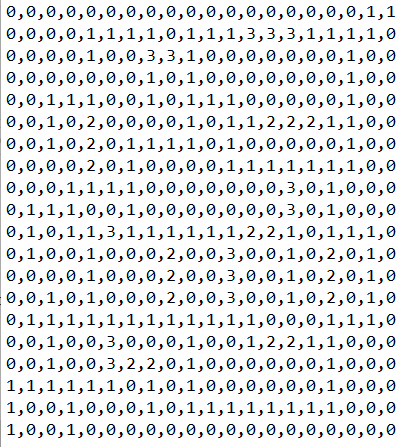
\includegraphics[scale=0.68]{Laberinto.png}}
\caption{Matriz que representa el laberinto usado, el inicio se ubica en la esquina inferior izquierda y el final en la superior derecha}
\label{Imagen de referencia}
\end{figure}

En cuanto a la representación del comportamiento de los robots, esta se realiza, como ya se mencionó, por medio de cadenas de Markov. Los estados de dicha cadena corresponde a enteros que almcenan el nivel de motor y batería, tipo de terreno de la celda actual y dirección del último movimiento realizado. La clave exacta de los estados, de aquí en adelante llamados "nodos", corresponde a: [1,2,3 - Terreno] [1,2,3 - Motor] [1,2,3 - Batería] [1 arriba, 2 abajo, 3 izquierda, 4 derecha], por lo que un robot con motor nivel 2 y batería nivel 1 que se acaba de mover a un terreno normal que ubicaba sobre él se encuentra en el estado 1211. Los estados para un robot dado en realidad solo cambian en cuanto a la última dirección dada y el terreno actual, pero debido a la necesidad de que todos los robots compartan un mismo diseño de cadena de Markov para el cruce, dicho diseño compartido incluye todos los posibles nodos. En cuanto a las probabilidades de pasar de un nodo a otro, de aquí en adelante "arcos", igualmente estan definidas para el producto cartesiano del conjunto de todos los nodos, aunque un robot dado solo se tomen en cuenta aquellas probabilidades correspondientes a los nodos que representen su motor y batería. La totalidad de la cadena de Markov se almacena en una estructura corresponde a un diccionario de \textit{Python} cuyas claves, los nodos, apuntan a un segundo diccionario con nuevamente un nodo por clave y por valor a la probabilidad de pasar del nodo de la clave del diccionario externo al nodo de la calve del diccionario interno. De lo anterior se puede deducir que la unidad cromósomica de la sección de genes de comportamiento del robot corresponde a entradas del diccionario externo.

Los robots almecenan muchos otros valores en sus atributos para ayudar a la ejecución del programa, tales como el hilo que se ejecuta para simbolizar su intento en el laberinto, su posición en dicho laberinto, su actual estado, los robots involucrados en el cruce que le dió origen, entre otros. En cuanto a la simulación del intento del robot en el laberinto, esta se realiza ejecuntado el hilo de cada robot antes mencionado. Dicho hilo consiste en la constante ejecución de una simulación de probabilidad entre las cuatro o menos probabilidades dadas por las cadenas de Markov propias de cada robot. Dichas probabilidades corresponden a los arcos entre el nodo que representa el estado actual y los tres o cuatro nodos que representan las tres o cuatro posbiles direcciones a tomar por el robot. El robot sigue realizando movimientos hasta que se agote su batería o hasta que alcance la salida del laberinto. 

En cuanto al diseño del algoritmo genético en sí, este se puede resumir en el diseño de los cromosomas, de la selección, del cruce y de la mutación. El algoritmo, a nivel de implementación, se encarga de crear generaciones de robots a partir de los procesos antes mencionados, y almacenarlas por medio de una lista de sus respectivos robots. Para cada una de estas generaciones se crea la cantidad de robots especificada a partir del cruce de la generación anterior (excepto la primer generación, la cual se confecciona a base de robots con propiedades aleatorias) y se ejecutan los hilos de cada uno de dichos robots, posteriormente se asignan los valores de adaptabilidad y se seleccionan los individuos a formar parte del cruce que da origen a la siguiente generación, no sin antes correr otra simulación de probabilidades para realizar las mutaciones que correspondan. La creación de nuevas generaciones se realiza hasta que se indique lo contrario por parte del usuario, ya que al mismo se le ve mostrando la adaptabilidad total de cada generación, es decir, la suma de los valores de adaptabilidad de todos sus individuos.

Ahora simplemente basta con hacer hincapié en los aspectos del algoritmo que quedan por discutir, es decir, la selección, el cruce y la mutación. En cuanto al cruce, este involucra dos procesos, la asginación de la adaptabilidad por medio de la función de adaptabildiad del algoritmo y la selección como tal de los individuos. La función de adaptabilidad asigna un valor flotante entre 0.1 y 100 a cada robot dependiendo de tres paramétros: la diferencia entre columnas y filas de la posición final del robot y la salida del laberinto, el costo, y el tiempo que le tomo al robot resolver el laberinto, representado por la cantidad de movimientos que se realizaron. Cabe resaltar que este último aspecto es ignorado en el caso de que el robot no logre salir del laberinto. Para ser más específico, la función adaptabilidad aplica la regla de tres sobre los tres aspectos anteriores, donde a la diferencia de columnas y filas se le asigna un máximo de 60 puntos si se tienen cero filas y columnas de diferencia (llego a la salida), al costo se le asigna un máximo de 20 puntos si se tiene el costo mínimo de 300 y al tiempo se le asigna un máximo de 20 puntos si el robot lograra resolver el laberinto sin hacer movimientos, lo cual es imposible pero permite crear una proporción comparativa para los valores reales. Una vez asignados los valores de adaptabilidad para todos los robots, estos se normlizan respecto a los valores del resto de la generación de modo que la adaptabilidad total relativa de toda la generación sea uno. La selección es un proceso mucho menos complejo, ya que simplemente involucra una simulación de probabilidad por cada miembro de la generación, ya que en cada corrida se elige un robot para participar en el cruce de acuerdo a la probabildiad representada en su adaptabilidad relativa, con la posibilidad de repetirse en la elección.

En cuanto al cruce, este se realiza independientemente para la sección de los genes correspondiente a hardware y la correspondiente a comportamiento. Cabe recordar que la primera de estas secciones corresponde a tres enteros que simbolizan los niveles de motor, batería y cámara (este último es siempre uno debido a la incompatibilidad con el diseño del comportamiento), mientras que la segunda corresponde a un diccionario externo con 108 entradas, cada una con a su vez 108 sub - entradas, en conjunto representado las 11664 probabilidades de paso entre nodos que rigen el movimiento del robot. Se toman los robots del cruce y emparejan entre sí una sola vez por selección en el caso de poblaciones pares y dos veces para el robot más apto en el caso de las impares. Posteriormente se selecciona un punto aleatorio en ambas secciones de los genes antes del cual se intercambian los enteros en el caso de la primera sección y los diccionarios internos en el caso de la segunda. Una vez realizado dicho intercambio, los dos nuevos cromosomas corresponden a dos robots de la siguiente generación, y así hasta que se generan una misma cantidad de robots para la próxima generación. Adicionamente, cada robot originado en el cruce almacena la información de aquellos robots que participaron en su cruce de origen. Como último paso de la iteración del algoritmo genético, se corre una probabilidad de mutación sobre cada robot que, de ser indicado por otra simulación de probabilidad, cambia un entero de la primera sección de los genes o un diccionario interno completo de la segunda sección por datos nuevos datos válidos pero aleatorios.

Una vez diseñadas todas las secciones del algoritmo, se programó una interfaz gráfica que permitiera visualizar el la adaptabilidad total (no la adaptabilidad relativa) alcanzada respecto a la cantidad de generaciones creadas hasta el momento. Además, dicha interfaz da la posibilidad de ver el robot con la mayor adaptabilidad alcanzada, así como visualizar el linaje de cualquier robot dado y detener la creación de nuevas generaciones cuando se desee.

\section{Análisis de resultados}

Se realizaron multiples corridas del algoritmo con una poblacion de 50 robots en cada generación y una probabilidad de mutación de 1 entre 100000 para tanto la mutacion de hardware como la de comportamiento. En Fig. 2 se puede apreciar uno ejemplo del resultado mas comun obtenido en las pruebas: la obtencion de una adaptabilidad total de alrededor de 2700 a partir de centesima generacion o antes. El estanque en una adaptabilidad total de 2700 se debe a la convergencia de genes alrededor de un ejemplar cuya adaptabilidad ronda los 60 puntos, en cuyo momento se entiende que se ha encontrado una solucion optima, mas aun tomando en cuenta que la adaptabilidad total de las primeras generaciones rondaba los 600 puntos.

\begin{figure}[htbp]
\centerline{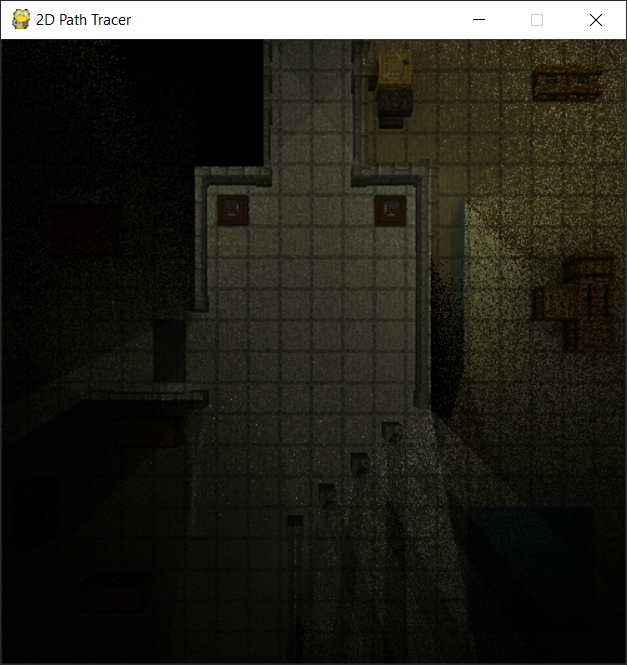
\includegraphics[scale=0.25]{Resultado1.png}}
\caption{Corrida con 100 generaciones}
\label{Imagen de referencia}
\end{figure}

No obstante, un aspecto que si varıo considerablemente entre corridas es la cantidad de generaciones que tomaba alcanzar el resultado de aproximadamente 3000 puntos de adabtabilidad total. En la Fig. 3 se puede apreciar un caso en el que tan pronto como a partir de la decimo segunda generacion se alcanzaba dicha adaptabilidad, con la solucion mas optima correspondiendo a un robot con 80 de adaptabilidad.

\begin{figure}[htbp]
\centerline{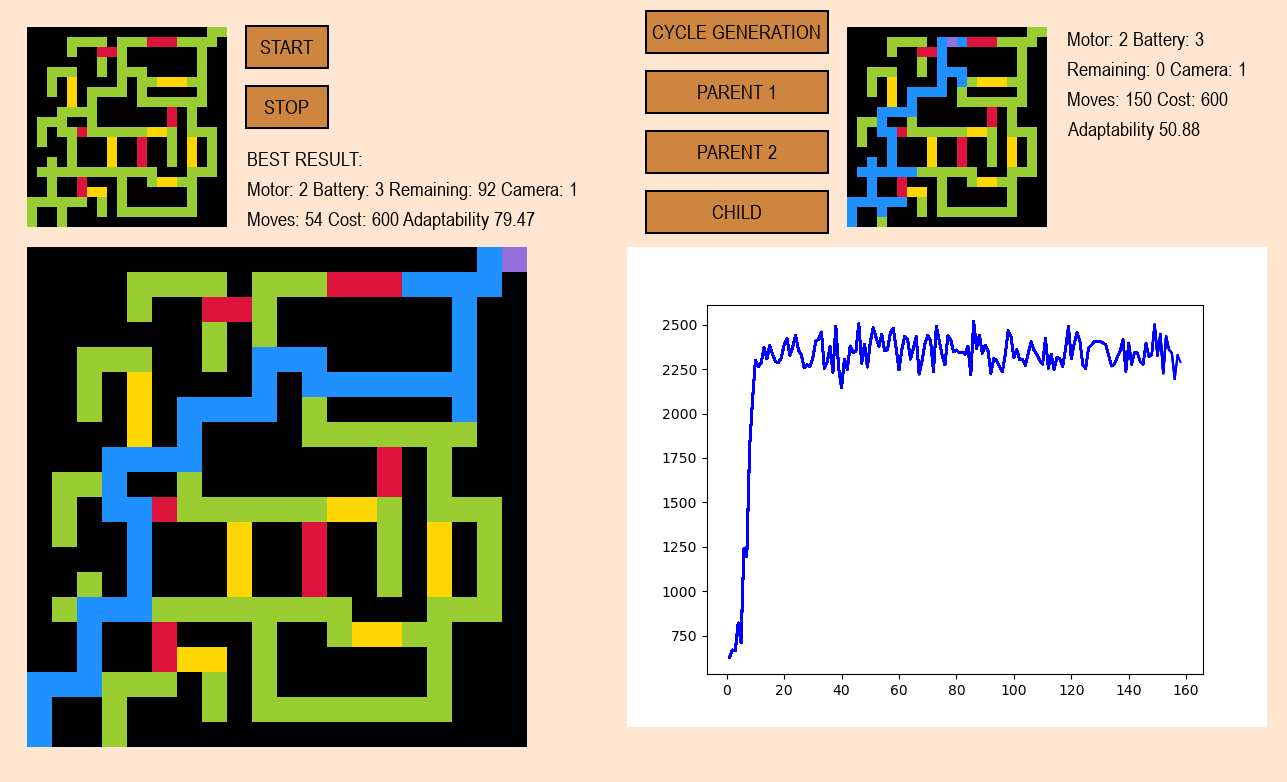
\includegraphics[scale=0.25]{Resultado2.png}}
\caption{Corrida con 160 generaciones}
\label{50 muestras completo}
\end{figure}

Cabe mencionar que, por medio de las pruebas aqui mostradas, se considera que queda probado el correcto funcionamiento del algoritmo genetico en la tarea de encontrar soluciones con un aproximado de 80 puntos de adaptabilidad.

\section{Conclusión}

Se concluye que se diseño satisfactoriamente un algoritmo genético capaz de dar una solucion óptima al problema dado, adicionalmente se cumplió con el objetivo de proveer al usuario una interfaz gráfica amigable para ver los datos de  la corrida de algoritmo. El único punto negativo al desarrollo del proyecto queda como la falta de la incorporación de la cámara a los genes de las soluciones.

\section{Acceso al proyecto}
El repositorio de GitHub en el cual se ubican todos los archivos empleados para el desarrollo de este proyecto puede ser accesado mediante el siguiente link: \url{https://github.com/TilapiaBoi/AnalisisPRY3}

\begin{thebibliography}{00}
\bibitem{b1} W. Hosch, \textit{Genetic algorithm}. Encyclopædia Britannica. n.d. Accesed on: Jul. 30, 2020. [Online]. Available: \url{https://www.britannica.com/technology/genetic-algorithm}
\bibitem{b2} S. Jaiswal, \textit{Markov Chains in Python: Beginner Tutorial}. Dec. 31, 2019. Accesed on: Jul 29, 2020. [Online]. Available: \url{https://www.datacamp.com/community/tutorials/markov-chains-python-tutorial}
\bibitem{b3} B. Unutmaz, \textit{Smart Boxes - Python AI Genetic Algorithm ( with Source Code )}, Sep. 25, 2019. Accessed on: Jul. 29,2020. [Video file]. Available: \url{ https://www.youtube.com/watch?v=GiaSEsZjWNc}
\bibitem{b4} W. Koehrsen, \textit{Markov Chain Monte Carlo in Python}. Feb. 9, 2018. Accesed on: Jul. 28, 2020. [Online]. Available:\url{https://towardsdatascience.com/markov-chain-monte-carlo-in-python-44f7e609be98}
\end{thebibliography}
\end{document}